\section{Business intelligence: generalità}
Trasformare i dati grezzi in informazioni
utilizzabili, da distribuire e condividere, creando così una conoscenza
collettiva della propria impresa.

\begin{itemize}
    \item E’ un processo analitico che trasforma i dati in informazioni
    a supporto della presa di decisioni ottimizzato da un
    insieme di tecnologie
    \item Con
    il fine di Migliorare i processi decisionali, di
    comunicazione e coordinamento delle interdipendenze
    aziendali, razionalizzare e ottimizzare il processo di Conoscenza
    creazione, gestione, diffusione e condivisione della
    conoscenza
\end{itemize}
\subsection{Business Intelligence: Leggere i dati per guidare le decisoni}

Fa uso di flussi di dati di qualsiasi dimensione per analizzare e visualizzare informazioni cruciali,
in relazione all'utilizzo che se ne intende fare.

Le aziende possono fare uso della BI per infromarsi sulle opzioni disponibili, permettendo di
migliorare la resa economica, l'efficienza, ecc.

La BI cerca di indivisuare e rendere percepibili i segnali nascosti contestualizzandoli.

Con la BI è possibile:
\begin{itemize}
    \item raccogliere dati
    \item classificare le informazioni
    \item analizzare i risulatati
    \item realizzare modelli predittivi
\end{itemize}

La BI si avvale di:
\begin{itemize}
    \item piattaforme dedicate
    \item modelli matematici, statistici e di analisi
    \item verifica dei risulatati
    \item esperti in materia
\end{itemize}

Si tratta di un percorso di valutazione supportato da strumenti di data visualizzation.
La BI è la chiave di lettura ottimale per capire cosa è successo e cosa sta succedendo,
offrendo soluzioni che aiutano a identificare schemi di comportamento significativi
e correlazioni tra le variabili entro un complesso insieme di dati, strutturati e non,
storici, attuali e potenziali.


Per avere una visione globale dell'azzienda, bisogna organizzare i dati in un unico rapporto.
Gli strumenti:
\begin{itemize}
    \item i report
    \item la dashboard(rappresentazioni dei dati graficamente)
    \item la dashboard rappresentano i \textbf{KPI}(Key Performance Indicator)
\end{itemize}

\subsubsection{Componenti della BI}
\begin{itemize}
    \item Dati: nozioni grezze
    \item informazioni: informazioni ottenute dai dati
    \item conoscenza: identificazioni di relazioni causa-effetto tra le infromazioni attraverso
    l'esperienza
\end{itemize}

\subsubsection{Gestione della conoscenza}
Creazione, raccolta e classificazione di informazioni provenienti da varie fonti
di dati che vengono distribuite ai vari utenti sulla base degli specifici interessi tramite
mezzi e strumenti diversi.

\subsubsection{Utenti nella BI}
\begin{enumerate}
    \item utente di alto livello: vista ampia e prende decisoni
    \item utenti specializzati: eseguono analisi dei dati
    \item lavoratori con necessità di report di base
    \item lavoratori senza report
\end{enumerate}

\begin{figure}[H]
    \centering
    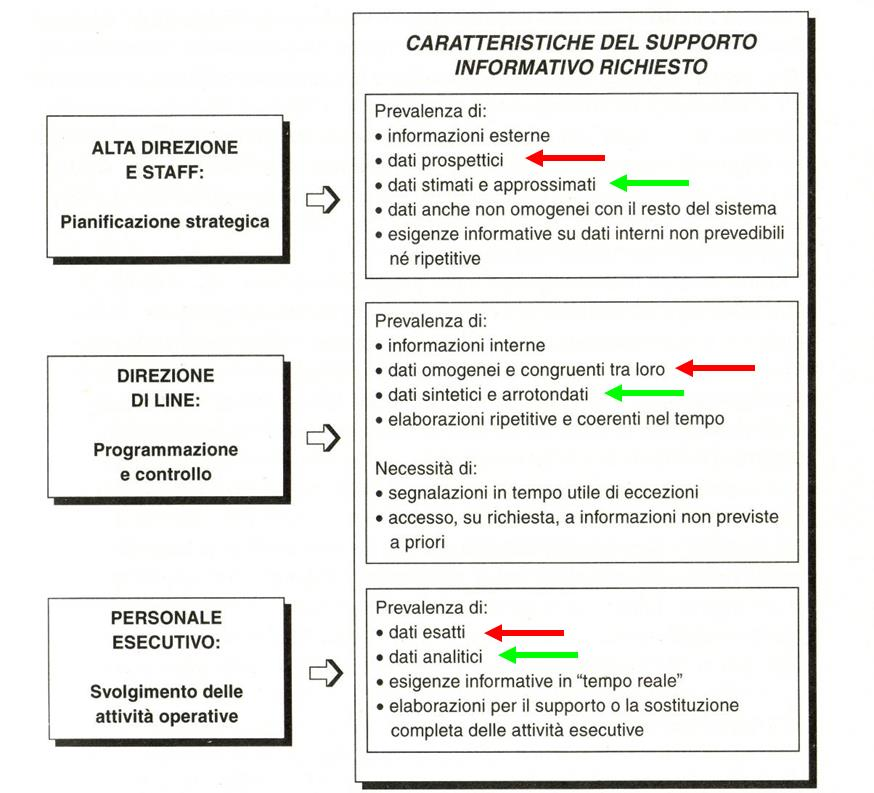
\includegraphics[width=0.4\linewidth]{imgs/2 - utenti BI}
    \label{fig:utenti_BI}
    \caption{Utenti nella BI}
\end{figure}


\subsection{Il valore della conoscenza}
\begin{figure}[H]
    \centering
    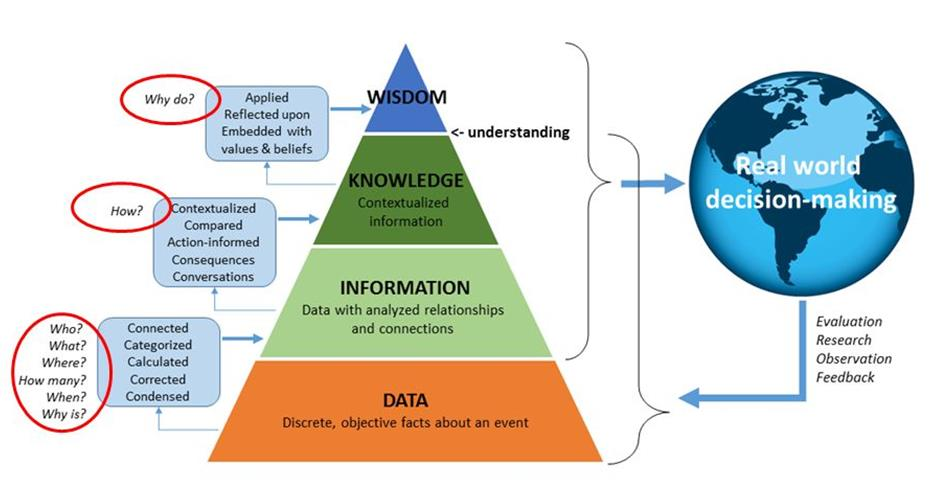
\includegraphics[width=0.6\linewidth]{imgs/3 - La piramide di DIKW}
    \label{fig:piramide_DIKW}
    \caption{Piramide di DIKW}
\end{figure}
\begin{itemize}
    \item Dati: nozioni grezze
    \item Informazioni: rappresentazione dei fatti (dati)
    organizzati in modo da essere comprensibili e
    significativi per l’utente destinatario
    \item Conoscenza: il collegamento fra più informazioni quali p.e.,
    l’identificazione di relazione causa-effetto
    tra informazioni attraverso esperienza, relazioni sociali etc.
    \item saggezza: capacità di aumentare l'efficacia. La saggezza aggiunge valore, il che
    richiede la funzione mentale che chiamiamo giudizio. I valori etici ed estetici che
    questo implica sono intrinseci all'attore e sono unici e personali. (Russell Ackoff)
\end{itemize}

\subsubsection{Ciò che genera conoscenza}
\begin{enumerate}
    \item Descriptive Analytics: l’insieme di strumenti orientati a descrivere la
    situazione attuale e passata dei processi aziendali e/o aree funzionali. Tali
    strumenti permettono di accedere ai dati secondo viste logiche flessibili e
    di visualizzare in modo sintetico e grafico i principali indicatori di
    prestazione
    \item Predictive Analytics, strumenti avanzati che effettuano l’analisi dei dati
    per rispondere a domande relative a cosa potrebbe accadere nel futuro;
    sono caratterizzati da tecniche matematiche quali regressione, forecasting,
    modelli predittivi, ecc
    \item Prescriptive Analytics, applicazioni big data avanzate che, insieme
    all’analisi dei dati, sono capaci di proporre al decision maker soluzioni
    operative/strategiche sulla base delle analisi svolte
    \item Automated Analytics, capaci di implementare autonomamente l’azione
    proposta secondo il risultato delle analisi svolte
\end{enumerate}

\subsection{Dati di qualità per essere affidabili}

I problemi:
\begin{itemize}
    \item dati in più posti
    \item dati non formattati per anali complesse
    \item diversi lavoratori operano su dati in maniera diversa
    \item quali dati dovrebbero essere esaminati
    \item interazione degli utenti
\end{itemize}

\subsection{Consolidamento dei dati}

\subsubsection{Pulizia dei dati}
I dati potrebbero essere incoerenti.
\subsubsection{Creare dati di qualità}
I dati puliti facilitano analisi più accurate.

\subsubsection{Estrazione, trasformazione e caricamento(ETL)}
Il processo di spostamento dei dati dai sistemi di origine, il consolidamento in una posizione centrale e la
correzzione delle incoerenze si chiama estrazione, trasformazione e consolidamento.

Il processo di ETL richiede l'$80\%$ del tempo.

\subsubsection{Datawarehouse}
I dati possono stare in posti diversi e fromati diversi, DB relazionali, fogli Excel ecc.
I Datawerehouse permettono di ottenere un layer di astrazzione, separando la provenienza dei dati dal loro utilizzo.

\begin{figure}[H]
    \centering
    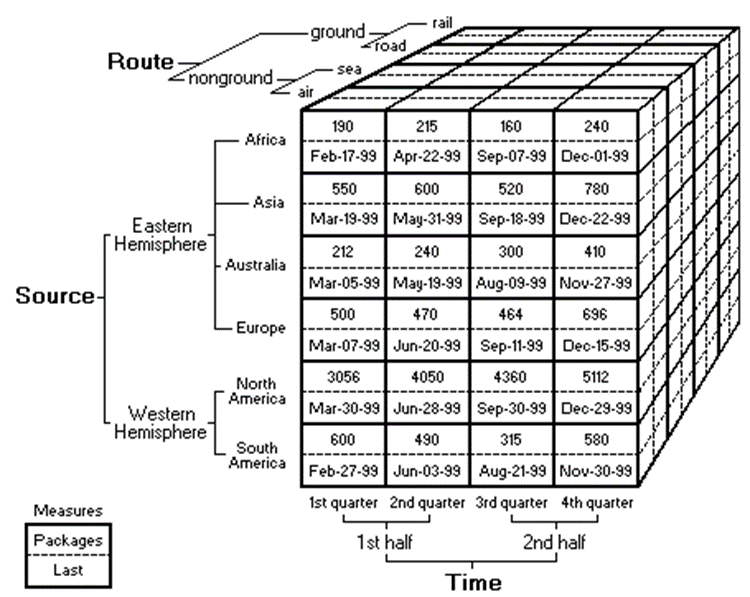
\includegraphics[width=0.4\linewidth]{imgs/4 - DWH}
    \label{fig:DWH}
    \caption{Cubo che compone il DWH}
\end{figure}

Il cubo è il componente base di un data werehouse, un DWH può contenere più cubi.


\subsubsection{OLAP}
Permette l'analisi dei dati su strutture che rendono le operazioni veloci e flessibili.

Tre categorie principali:
\begin{itemize}
    \item MOLAP
    \begin{itemize}
        \item più usati
        \item ha un motore specifico per l'analisi
        \item crea le dimensione con un misto di dettaglio e astrazione
        \item veloce
    \end{itemize}
    \item ROLAP
    \begin{itemize}
        \item lavora sui DB relazionali
        \item minor spazio su disco e ram
        \item più lento
    \end{itemize}
    \item HOLAP
    \begin{itemize}
        \item lavora con DB relazionali
        \item più veloce dei ROLAP
        \item più scalabile dei MOLAP
    \end{itemize}
\end{itemize}

Le principali operazioni negli OLAP sono:
\begin{itemize}
    \item PIVOTING
    \begin{figure}[H]
        \centering
        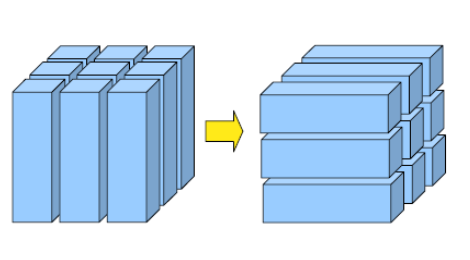
\includegraphics[width=0.2\linewidth]{imgs/5 - pivoting}
        \label{fig:pivoting}
        \caption{Pivoting}
        è l'operazione di rotazione delle dimensioni di analisi. È un'operazione
        fondamentale per analizzare totali ottenuti in base a dimensioni diverse o
        se si vogliono analizzare aggregazioni trasversali.
        La tabella pivot è la reportistica che risulta da una query OLAP elaborata
        su dati organizzati all'interno di un ipercubo OLAP
    \end{figure}
    \item SLICING
    \begin{figure}[H]
        \centering
        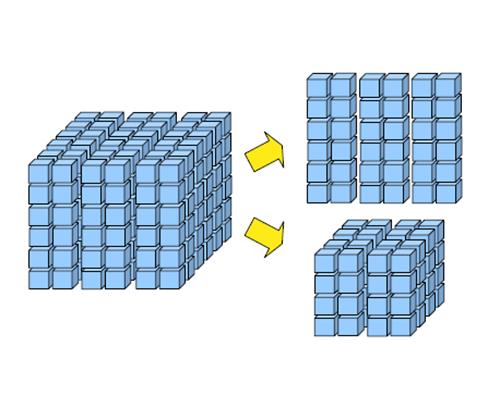
\includegraphics[width=0.2\linewidth]{imgs/6 - slicing - dicing}
        \label{fig:slicing-dicing}
        \caption{Slicing e Dicing}
        Si fissa uno specifico valore per una delle
        dimensioni del "cubo", estraendo quindi una
        "fetta" e ottenendo un nuovo cubo con una
        dimensione in meno rispetto a quello di
        partenza
    \end{figure}
    \item DICING
    Si focalizza l’analisi su un sottoinsieme del
    "cubo" avente particolare interesse per
    l'analista
    \item DRILL-DOWN
    \begin{figure}[H]
        \centering
        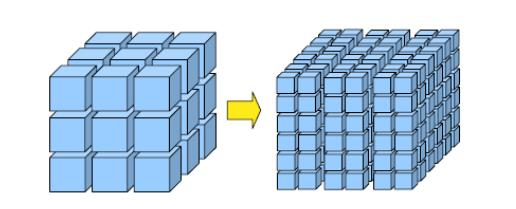
\includegraphics[width=0.3\linewidth]{imgs/7 - drill down}
        \label{fig:drill_down}
        \caption{Drill-down}
    \end{figure}
    è l'operazione di "esplosione" del dato nelle sue determinanti.
    L'operazione di drill-down può essere eseguita seguendo due diversi
    percorsi: la gerarchia costruita sulla dimensione di analisi (p. es.:
    passaggio dalla famiglia di prodotti all'insieme dei prodotti che ne fanno
    parte) oppure la relazione matematica che lega un dato calcolato alle sue
    determinanti (p. es.: passaggio dal margine al ricavo e costo che lo
    generano).
\end{itemize}


\subsubsection{Data mining}
Estrazione di conoscenza da banche grandi banche dati tramite algoritmi che individuano
le associazioni nascoste tra le informazioni e le rendono disponibili.

Con il data mining si intende l'applicazione di una o più tecniche che consentono l'esplorazione
di grandi quantità di dati, con l'obbiettivo di individuare le informazioni più significative.


Un processo di base consiste in:
\begin{enumerate}
    \item definizione dell'obbiettivo
    \item indivisuazione delle fonti
    \item estrazione dei dati
    \item pre-processing
    \item data mining
    \item interpretazione
    \item reppresentazioni dei risultati
\end{enumerate}

Tipologia di problemi ai quali il data mining fonisce una risposta:
\begin{itemize}
    \item Classificazione: definizione delle caratteristiche del data set
    \item Clustering: identificazione delle affinità che definiscono i gruppi
    \item Sequencing: identificazioni delle correlazioni in un periodo definitp
    \item associazione: identificazione delle correlazioni tra comportamenti
    \item Previsione: identificazioni di trend
\end{itemize}

\begin{figure}[H]
    \centering
    
\includegraphics[width=0.7\linewidth]{imgs/8 - dataming}
    \label{fig:data_mining_domande}
    \caption{Domande DM}
\end{figure}

\subsection{Osseviamo i dati}
Attualmente ci sono quantità di dati quasi infiniti prodotti quotidianamente,
bisogna darci un senso\ldots

\subsubsection{Le fonti}

\begin{itemize}
    \item Interne
    Fonti operazionali, dati sul business interno ecc
    \item Esterne
    analisi dei sentiment, ecc
\end{itemize}
\subsubsection{Aspetto}

\begin{itemize}
    \item Dati quantitativi
    descritti tramite numeri
    \item Dati qualitativi
    non rappresentati dal valore numerico
\end{itemize}

\subsubsection{Struttura}
\begin{itemize}
    \item Dati strutturati
    dati ordinati in una struttura
    \item Dati non strutturati
    formato libero
    \item Dati semi strutturati
\end{itemize}

Il $90\%$ dei dati sono in un formato difficile per l'elaborazione.

\subsubsection{I quattro livelli dei dati}
\begin{itemize}
    \item Livello nominale
    Dati descritti unicamente per nome e categoria.
    Per trovare il centro dei dati si considera la moda.
    \item livello ordinale
    Esiste unìordine di valutazione, utile all'ordinamento e al confronto.
    SI utilizza la mediana.
    \item livello degli intervalli
    i dati di questo tipo consentono di eseguire sottrazioni fra i punti dei dati.
    Si usa la media.
    \item livello dei rapporti
    I dati al livello intervalli non hanno un valore nullo o zero, sui dati dei rapporti si possono fare
    moltiplicazioni e divisioni.
    La media imane topppp.
\end{itemize}


\subsection{Dara science Vs Business Intelligence}
\subsubsection{BI}
\begin{itemize}
    \item fondamentale l'uso di tecnologie e processi dalle aziende per l'anili dei dati
    \item esegue la conversione da dati grezzi a informazioni
    \item anali dei dati strutturati per aprendere conoscenza
    \item supporta il processo decisionale basato sui fatti
    \item ha un impatto direttosulle decisione delel aziende
    \item nuove opportunità per l'azienda
\end{itemize}

\subsubsection{Data science}
\begin{itemize}
    \item fondamentale un campo in cui la conoscenza venga estratta dai dati usando vari metodi e algoritmi
    \item combinazione di vari strumenti matematici, algoritmi, statistica, e tecnologie di apprendimento automatico
    \item sia dati strutturati che non
    \item implica lo studio delle tendenze attuali e prevede le future
\end{itemize}


\subsubsection{Analisi con BI}
\begin{itemize}
    \item BI lavora su una formula preesistente
    \item l'azienda contatta un esperto di BI con i dati e le formule e si aspetta un risultato definito
\end{itemize}
\subsubsection{Anali con DS}
\begin{itemize}
    \item Si parte da una domanda
    \item non si utilizza la solita formula
    \item La Sciena dei dati cerca di anticipare il futuro
\end{itemize}

\begin{figure}[H]
    \centering
    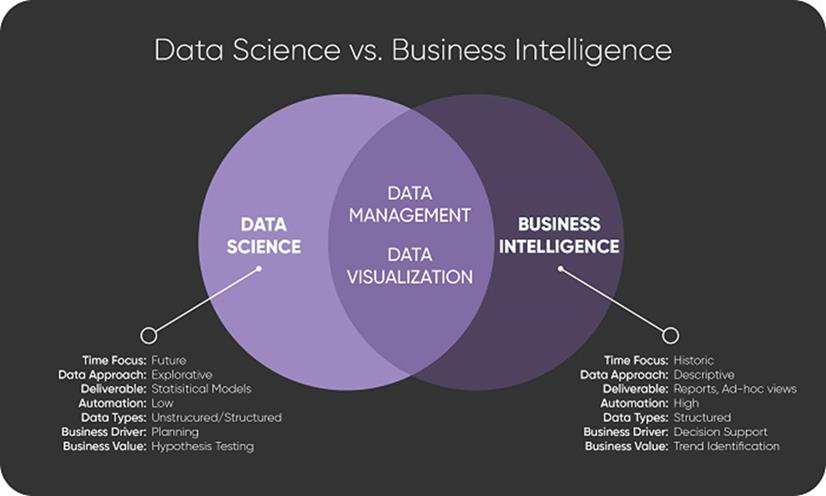
\includegraphics[width=0.8\linewidth]{imgs/10 - BI VS DS}
    \label{fig:data_science_vs_business_intelligence}
    \caption{Data Science VS Business Intelligence DM}
\end{figure}